\chapter{Introducción}
\label{chap:introduccion}

\section{Contextualización}
 El área de aplicación específica para este proyecto es la carrera de Ingeniería en Tecnologías de la Información, donde se ha identificado que la gestión de la información académica para los estudiantes es predominantemente estática. Actualmente, el acceso a datos críticos sobre mallas curriculares, requisitos de graduación o perfiles profesionales depende de la navegación manual por el sitio web institucional o de la lectura de extensos archivos PDF, lo que deriva en una experiencia de usuario pasiva y demorada.

El entorno universitario actual demanda canales de comunicación más ágiles que respondan a la necesidad de inmediatez de los estudiantes. La situación identificada revela una brecha entre la disponibilidad de la información y la facilidad con la que el usuario puede obtener respuestas precisas a sus inquietudes. Esta dispersión documental no solo dificulta la orientación de los alumnos de nuevo ingreso, sino que también genera una carga de consultas repetitivas que podrían automatizarse. En este contexto, surge la necesidad de modernizar estos puntos de contacto, transformando los repositorios de datos tradicionales en un entorno de consulta dinámico y proactivo que aproveche las tendencias actuales en interfaces humano-computadora.


%La implementación de este asistente virtual inteligente se aplicará como un punto de contacto estratégico dentro del campus, afectando positivamente la interacción entre los estudiantes y la documentación de la universidad. Al integrar un avatar 3D equipado con visión artificial y procesamiento de lenguaje natural, el sistema permitirá que la comunidad estudiantil acceda a la información de su carrera de forma conversacional y visual. Esto elimina la necesidad de realizar búsquedas manuales exhaustivas en plataformas digitales complejas, proporcionando una solución innovadora que centraliza el conocimiento académico y mejora significativamente la experiencia del estudiante al ofrecer un servicio de orientación rápido, intuitivo y tecnológicamente avanzado.


\section{Estado del Arte}

El presente estado del arte fundamenta la conceptualización, diseño y desarrollo de un Asistente Virtual Inteligente enfocado en la difusión proactiva de información académica para los estudiantes de la carrera de Tecnologías de la Información (TI). Para abordar la complejidad tecnológica y el impacto institucional de esta solución, esta sección se estructura en cuatro dimensiones analíticas principales.

En primer lugar, se presenta un diagnóstico del funcionamiento actual del sistema de información en la Universidad Tecnológica Indoamérica, identificando las fricciones en la experiencia del usuario. En segundo lugar, se expone la evolución tecnológica de los asistentes virtuales, destacando la transición hacia interfaces antropomórficas, como los avatares 3D, y la integración de la visión artificial. En tercer lugar, se analiza la adopción actual de estas tecnologías en diversas instituciones de educación superior en el Ecuador, estableciendo un contexto nacional. Finalmente, la sección concluye con un análisis comparativo exhaustivo que contrasta quince proyectos y referentes científicos similares con la propuesta de esta investigación.

\subsection{Diagnóstico del Sistema de Información Institucional en la Universidad Tecnológica Indoamérica}
Para que la implementación de un asistente virtual sea pertinente y genere un impacto medible, debe resolver problemas operativos específicos dentro de su entorno de despliegue. En la Universidad Tecnológica Indoamérica (UTI), la administración y difusión de la información académica y curricular se gestiona primordialmente a través de su Sistema de Gestión Académica (SGA).

Actualmente, cuando un estudiante de la carrera de TI requiere consultar su avance de malla curricular, prerrequisitos de asignaturas o normativas de titulación, debe autenticarse en el portal web del SGA mediante credenciales de acceso. Una vez dentro, la recuperación de la información se realiza navegando por diversos menús que, en su mayoría, derivan en la generación de reportes en formato PDF estático, diseñados idealmente para su impresión. Este modelo de interacción representa un paradigma de recuperación de información lineal y pasivo; si el estudiante presenta dudas de interpretación sobre la secuenciación de materias, el documento no ofrece retroalimentación dinámica, obligando al alumno a buscar asistencia presencial, lo que genera demoras y sobrecarga de consultas administrativas repetitivas.

De manera contrastante, la Universidad Indoamérica posee un entorno altamente propicio para la innovación tecnológica. La institución impulsa activamente la investigación aplicada en inteligencia artificial y oferta programas académicos de posgrado especializados en IA, innovación empresarial y desarrollo de entornos virtuales. En este contexto, el prototipo de asistente virtual propuesto no busca reemplazar la infraestructura del SGA, sino acoplarse como una capa de interfaz moderna, transformando los repositorios de datos tradicionales en un canal de servicio inmediato, conversacional y proactivo.

\subsection{Evolución Tecnológica: Asistentes Virtuales, Avatares 3D y Visión Artificial}
La evolución de las interfaces humano-computadora en el ecosistema educativo ha transitado desde chatbots transaccionales basados puramente en texto hacia agentes conversacionales encarnados o multimodales. Si bien los modelos basados en texto logran automatizar respuestas, la evidencia empírica en la educación superior subraya que la dotación de características antropomórficas a los sistemas facilita la creación de entornos centrados en el estudiante, promoviendo la empatía y la presencia social \cite{robinson2024ai}.

La integración de Modelos de Lenguaje Grande (LLM) dota al sistema de comprensión semántica, mientras que plataformas de middleware proporcionan la materialización visual. Estas plataformas permiten la generación de avatares 3D de alta fidelidad, equipados con mallas faciales configuradas para soportar animaciones expresivas y sincronización labial en tiempo real, lo que reduce la carga cognitiva y humaniza el proceso de difusión de la información \cite{pabon2025naia}.

Simultáneamente, la visión artificial (\textit{Computer Vision}) ha transformado a estos asistentes de respondedores pasivos a sistemas capaces de interpretar señales visuales básicas de interacción. Mediante algoritmos de aprendizaje profundo, redes neuronales convolucionales y extracción de puntos de referencia faciales (\textit{landmarks}), un asistente con interfaz de avatar puede adaptar su comportamiento visual, orientar su mirada simulada y mejorar la naturalidad de la comunicación con el usuario \cite{lightweightgaze2024}.

No obstante, la literatura reciente enfatiza la extrema precaución ética que requiere el uso de señales visuales en entornos educativos. Este antecedente dicta un mandato de ``privacidad por diseño'' para la presente tesis: los algoritmos de visión artificial deben procesar la información de manera efímera, sin almacenar imágenes ni identificar personalmente al alumno sin su consentimiento expreso \cite{abedi2024engagement}.

\subsection{Adopción de Inteligencia Artificial en Universidades del Ecuador}
El análisis del estado del arte demuestra un creciente interés por la automatización de procesos académicos en las instituciones de educación superior del Ecuador. Diversas universidades se encuentran en etapas de investigación o implementación de soluciones basadas en inteligencia artificial que sirven como antecedentes directos para este proyecto:

\begin{itemize}
    \item \textbf{Universidad Técnica Particular de Loja (UTPL):} Investigadores de esta institución han desarrollado propuestas de asistentes virtuales desplegados mediante tecnología holográfica para optimizar los servicios estudiantiles y reducir tiempos de espera \cite{caceres2024asistente}. Además, la universidad ha liderado proyectos de realidad extendida, implementando un ``Campus 3D'' donde los usuarios navegan a través de avatares.
    \item \textbf{Universidad Politécnica Salesiana (UPS):} Implementó un asistente virtual fundamentado en procesamiento de lenguaje natural y aprendizaje automático, mediante redes neuronales recurrentes, para gestionar eficientemente la comunicación con aspirantes a estudios de posgrado a través de canales de mensajería, optimizando los recursos administrativos \cite{guncay2022desarrollo}.
    \item \textbf{Pontificia Universidad Católica del Ecuador (PUCE):} Con el respaldo de su grupo de investigación en inteligencia artificial, se desarrolló ``TELIA'', un asistente virtual integrado en Microsoft Teams para automatizar y transformar digitalmente la resolución de problemas en las mesas de servicios tecnológicos \cite{telia2024}.
    \item \textbf{Escuela Superior Politécnica del Litoral (ESPOL):} Se diseñó una plataforma web con un asistente virtual basado en IA y modelos de \textit{machine learning}, como Random Forest, capaz de interpretar preguntas en lenguaje natural para proporcionar indicadores de desempeño predictivos, reduciendo los tiempos de consulta de casi una hora a once minutos \cite{diaz2025asistente}.
    \item \textbf{Universidad Internacional del Ecuador (UIDE) y Universidad Tecnológica ECOTEC:} Ambas instituciones se encuentran a la vanguardia de la innovación educativa nacional. UIDE fomenta ecosistemas académicos enriquecidos por IA, mientras que ECOTEC utiliza tecnologías avanzadas, incluyendo sistemas de reconocimiento facial para el acceso seguro al campus y el uso de internet de las cosas.
\end{itemize}

\subsection{Análisis Comparativo de Soluciones y Proyectos Similares}
A continuación, la Tabla~\ref{tab:comparativa} expone un contraste analítico entre el prototipo propuesto en esta investigación y diversos referentes bibliográficos y tecnológicos de relevancia, detallando sus objetivos, metodologías de interfaz y el uso de la visión computacional.

\clearpage
\begin{landscape}
\footnotesize
\setlength{\LTleft}{0pt}
\setlength{\LTright}{0pt}
\setlength{\LTcapwidth}{\linewidth}
\setlength{\tabcolsep}{3pt}
\renewcommand{\arraystretch}{1.18}
\begin{longtable}{|>{\raggedright\arraybackslash}p{3.2cm}|>{\raggedright\arraybackslash}p{3.9cm}|>{\raggedright\arraybackslash}p{3.5cm}|>{\raggedright\arraybackslash}p{3.5cm}|>{\raggedright\arraybackslash}p{5.8cm}|}
\caption{Comparativa del Proyecto Propuesto frente al Estado del Arte.}\label{tab:comparativa}\\
\hline
\rowcolor[HTML]{EFEFEF}
\textbf{Proyecto / Autores} & \textbf{Objetivo principal} & \textbf{Interfaz de usuario} & \textbf{Uso de visión artificial} & \textbf{Diferencia principal con el proyecto propuesto} \\ \hline
\endfirsthead

\hline
\rowcolor[HTML]{EFEFEF}
\textbf{Proyecto / Autores} & \textbf{Objetivo principal} & \textbf{Interfaz de usuario} & \textbf{Uso de visión artificial} & \textbf{Diferencia principal con el proyecto propuesto} \\ \hline
\endhead

\hline
\multicolumn{5}{r}{\textit{Continúa en la siguiente página}} \\
\endfoot

\hline
\endlastfoot

\textbf{Proyecto Propuesto (Tesis TI - Indoamérica)} & Transformar la consulta documental de mallas y normativas en una experiencia dinámica y ágil. & Avatar 3D + procesamiento de lenguaje natural por voz. & Análisis visual no biométrico para apoyar la interacción del avatar. & Especializado en la resolución de la fricción documental específica de la carrera de TI, uniendo gestión curricular con una interfaz multimodal de orientación académica. \\ \hline
\textbf{NAIA Framework} \\ \cite{pabon2025naia} & Asistencia académica general mediante una arquitectura de cinco roles. & Avatar 3D (Ready Player Me) + modelos LLM. & Analiza el entorno visual para retroalimentar la interacción. & NAIA abarca procesos generales para toda la universidad; la propuesta actual acota el razonamiento a normativas de TI, evitando respuestas ambiguas. \\ \hline
\textbf{EverydAI} \\ \cite{everydai2025} & Asistencia en la toma de decisiones cotidianas, como cocina, moda y fitness. & Avatar 3D diferenciado por dominio de conocimiento. & Detección de objetos físicos en tiempo real. & Está orientado al entorno doméstico; el proyecto adapta esa capacidad multimodal proactiva al ecosistema burocrático universitario. \\ \hline
\textbf{Asistente Holográfico UTPL} \\ \cite{caceres2024asistente} & Responder consultas frecuentes para servicios estudiantiles. & Despliegue mediante holograma. & No reporta visión proactiva para interacción autónoma. & Utiliza proyección holográfica reactiva; la tesis propone un avatar 3D integrado a un prototipo software de orientación académica. \\ \hline
\textbf{Asistente Posgrado UPS} \\ \cite{guncay2022desarrollo} & Reducir la carga de admisiones mediante respuestas automatizadas. & Interfaz textual vía WhatsApp y Messenger. & No utiliza visión artificial. & Es un sistema pasivo basado en texto; el proyecto propuesto humaniza el servicio al dar un rostro y voz 3D a la institución. \\ \hline
\textbf{TELIA Mesa Ayuda PUCE} \\ \cite{telia2024} & Automatización de soporte y tickets tecnológicos. & Chatbot integrado en Microsoft Teams. & No utiliza visión artificial. & Es una solución transaccional corporativa; la tesis propone un agente de difusión académica con representación visual mediante avatar 3D. \\ \hline
\textbf{Asistente Desempeño ESPOL} \\ \cite{diaz2025asistente} & Proporcionar métricas predictivas industriales. & Plataforma web conversacional. & No utiliza visión artificial. & Mantiene un enfoque predictivo de datos tabulares, sin elementos de presencia social ni contexto espacial. \\ \hline
\textbf{GPTAvatar} \\ \cite{robinson2024ai} & Crear un entorno educativo inmersivo de código abierto. & Avatar 3D en motor gráfico Unity. & No se enfoca en la detección física del entorno del usuario. & Es una herramienta generalista; el proyecto de tesis se orienta a un servicio institucional sustentado en bases documentales específicas. \\ \hline
\textbf{Control de Mirada ECAs} \\ \cite{lightweightgaze2024} & Mejorar la toma de turnos en espacios públicos ruidosos. & Agente conversacional en pantalla. & Detección del orador activo para dirigir la mirada del avatar. & El estudio se enfoca en el algoritmo visual-acústico; la tesis es una plataforma integral de recuperación de información. \\ \hline
\textbf{Medición de Compromiso} \\ \cite{abedi2024engagement} & Medir niveles de atención en educación virtual. & Modelo analítico sin interfaz avatar definida. & Redes ST-GCN y \textit{landmarks} faciales. & Es un algoritmo aislado; el proyecto propuesto puede integrar estas lógicas para adaptar dinámicamente la explicación del avatar. \\ \hline
\textbf{Asistente de Tesis UPN} \\ \cite{laureano2022asistente} & Apoyar la estructuración metodológica de trabajos de grado. & Chatbot de texto basado en IA. & No utiliza visión artificial. & Apoya la generación de contenido investigativo; el proyecto propuesto no interviene en tareas, sino en la burocracia administrativa. \\ \hline
\textbf{Simulaciones Médicas UMH} \\ \cite{fernandez2022virtual} & Entrenamiento diagnóstico para estudiantes de medicina. & Avatar 3D de paciente clínico. & No implementa visión artificial proactiva. & La interacción se orienta a evaluación de competencias, frente a la naturaleza informativa y guiada de la propuesta de TI. \\ \hline
\textbf{TalkMateAI} \\ \cite{talkmateai2023} & Desarrollar un compañero de IA multimodal de ejecución local. & Avatar 3D web. & Modelos visión-lenguaje ligeros. & Es una arquitectura técnica de código abierto; la tesis adopta estos principios de baja latencia para un caso de uso académico real. \\ \hline
\textbf{AI Desktop Assistant} \\ \cite{karagond2024ai} & Mejorar la interacción mediante reconocimiento visual de escritorio. & Asistente en PC. & Reconocimiento visual de gestos y objetos mediante webcam. & Está orientado al control del sistema operativo, a diferencia de la orientación a servicios curriculares del prototipo de tesis. \\ \hline
\textbf{Modelo Alerta Transporte} \\ \cite{cardenas2024modelo} & Prevención de aglomeraciones mediante detección visual. & Interfaz de administración de alertas. & Detección de altas concentraciones de personas. & Está orientado a seguridad y flujos masivos; el proyecto propuesto utiliza la detección para iniciar un diálogo uno a uno de manera empática. \\ \hline
\end{longtable}
\normalsize
\end{landscape}

\section{Planteamiento del Problema}
%textit{[Definir de forma clara y precisa el problema o brecha tecnológica identificada. Describir las causas que lo originan y los efectos que genera en el contexto analizado. No incluir la solución en esta sección.]}
En el actual ecosistema de educación superior, la inmediatez y la accesibilidad a la información son factores determinantes para el éxito y la retención estudiantil. En la carrera de Ingeniería en Tecnologías de la Información de la Universidad Tecnológica Indoamérica, se ha identificado una brecha tecnológica significativa en la capa de interacción entre los estudiantes y los repositorios de información institucional. 

Actualmente, la gestión de datos académicos críticos tales como mallas curriculares, requisitos de titulación, procesos de prácticas preprofesionales y perfiles de egreso se realiza a través de un modelo predominantemente estático. Las causas de esta problemática radican en que los sistemas de información heredados fueron diseñados bajo un paradigma de almacenamiento y lectura lineal, obligando al estudiante a navegar manualmente por múltiples menús del sitio web institucional o a descargar y leer extensos archivos en formato PDF. 

Los efectos de esta infraestructura recaen directamente sobre la experiencia del usuario, volviéndola pasiva, cognitivamente exhaustiva y demorada. Esta dispersión documental dificulta severamente la orientación autónoma, especialmente para los alumnos de nuevo ingreso. Ante la incapacidad de los documentos estáticos para resolver dudas de interpretación o casos específicos, los estudiantes se ven forzados a recurrir a la atención presencial. En consecuencia, se genera un cuello de botella operativo, sobrecargando al personal administrativo y docente con un alto volumen de consultas repetitivas que, bajo un esquema tecnológico adecuado, son inherentemente automatizables. 



\section{Justificación}
%\textit{[Redactar un texto argumentativo que exponga la importancia del proyecto, su impacto técnico y operativo, la utilidad de la solución, los beneficiarios directos e indirectos y la factibilidad técnica y operativa de su implementación.]}

La modernización de los canales de comunicación universitaria es un imperativo frente a una generación de estudiantes nativos digitales que demandan respuestas ágiles e interactivas. Este proyecto se justifica por su capacidad para transformar un modelo de consulta obsoleto en una experiencia dinámica, centralizada y tecnológicamente inmersiva mediante la implementación de un Asistente Virtual Inteligente.

A nivel técnico y operativo, la incorporación de Procesamiento de Lenguaje Natural (PLN), visión artificial no biométrica y un avatar 3D permite crear una interfaz de consulta más natural e intuitiva. En lugar de obligar al estudiante a recorrer documentos extensos o menús institucionales, el sistema interpreta consultas en lenguaje natural y presenta respuestas contextualizadas, mejorando la asimilación de la información gracias al componente visual y conversacional del avatar.

La utilidad de la solución radica en su capacidad de operar de manera continua y estandarizada, asegurando que la información entregada sobre la carrera de TI sea siempre precisa y actualizada. Los beneficiarios directos de este proyecto son los estudiantes de la carrera, quienes obtendrán una herramienta de orientación intuitiva y resolutiva. Como beneficiarios indirectos, el personal administrativo y académico verá reducida la carga de atención de consultas rutinarias, permitiéndoles enfocar sus esfuerzos en tareas de mayor valor institucional. Además, el proyecto posiciona a la Universidad Indoamérica a la vanguardia en la adopción de interfaces humano-computadora avanzadas.

Finalmente, la ejecución de este proyecto es factible tanto a nivel técnico como operativo. Como estudiante de la carrera de TI, se cuenta con los conocimientos de desarrollo de software necesarios, y actualmente existen frameworks de inteligencia artificial, APIs de síntesis de voz, librerías de visión artificial y plataformas de creación de avatares que son altamente accesibles para integrarse en un prototipo funcional de software.

\section{Objetivos}
\subsection{Objetivo General}
Desarrollar un prototipo de Asistente Virtual Inteligente, provisto de una interfaz de avatar 3D y visión artificial, para optimizar la difusión proactiva y el acceso a la información académica de los estudiantes en la carrera de Ingeniería en Tecnologías de la Información de la Universidad Tecnológica Indoamérica.

%\textit{[Redactar el propósito principal del proyecto, alineado con la solución propuesta e incluyendo explícitamente su implementación.]}
\subsection{Objetivos Específicos}
\begin{itemize}
    \item \textbf{Analizar} los procesos actuales de gestión y consulta de documentación académica en la institución para determinar los requerimientos funcionales, no funcionales y la base de conocimiento conversacional del sistema.
    \item \textbf{Diseñar} la arquitectura de software del asistente, definiendo la integración del módulo conversacional, el motor de Procesamiento de Lenguaje Natural (PLN), la base de conocimiento académica y el entorno gráfico del avatar 3D.
    \item \textbf{Implementar} el prototipo del asistente virtual integrando los modelos de inteligencia artificial, la interfaz antropomórfica y los mecanismos de interacción visual no biométrica en un entorno de software controlado.
    \item \textbf{Evaluar} el desempeño, precisión y usabilidad del prototipo mediante pruebas de interacción con estudiantes de la carrera, midiendo indicadores como la reducción de tiempos de consulta y el nivel de aceptación del usuario.
\end{itemize}
%\textit{[Enumerar acciones concretas, medibles y verificables que permitan alcanzar el objetivo general. Los objetivos deben cubrir análisis, diseño, implementación y validación.]}

\section{Alcance del Proyecto}
%\textit{[Delimitar los límites del proyecto, especificando claramente los componentes, módulos o funcionalidades que se incluyen, así como aquellos que se excluyen.]}

El proyecto comprende el diseño, desarrollo y validación de un prototipo funcional de asistente virtual, orientado exclusivamente a los estudiantes de la carrera de Tecnologías de la Información.

\textbf{Componentes y funcionalidades incluidas:}
\begin{itemize}
    \item \textbf{Módulo de Visión Artificial:} Integración de mecanismos visuales no biométricos para apoyar la interacción del avatar, sin identificar personalmente al usuario ni condicionar el funcionamiento del sistema a infraestructura física específica.
    \item \textbf{Módulo Conversacional (PLN):} Implementación de un motor de Inteligencia Artificial capaz de comprender y procesar solicitudes orales en lenguaje natural (Speech-to-Text), procesar la respuesta mediante un Modelo de Lenguaje Grande (LLM) contextualizado con la información de la carrera (mallas, reglamentos), y emitir una respuesta en audio (Text-to-Speech).
    \item \textbf{Interfaz de Avatar 3D:} Desarrollo de una interfaz gráfica que integre un avatar antropomórfico con capacidad de sincronización labial (\textit{lip-sync}) en tiempo real, generando una interacción inmersiva.
\end{itemize}

\textbf{Límites y exclusiones:}
\begin{itemize}
    \item El sistema \textbf{no} realizará reconocimiento facial biométrico para la identificación personal del estudiante, preservando la privacidad y operando de forma anónima (Privacidad por Diseño).
    \item El asistente \textbf{no} tendrá integración transaccional directa con la base de datos del Sistema de Gestión Académica (SGA) para realizar acciones como matriculación, pago de aranceles o modificación de notas. Su función será estrictamente informativa y de orientación.
    \item \textbf{No} se desarrollará una versión de aplicación móvil ni despliegue web masivo; el alcance tecnológico se delimita a una prueba de concepto funcional en un entorno de software controlado.
\end{itemize}

\section{Fundamentación Teórica}
%\textit{[Desarrollar los fundamentos teóricos, conceptos, modelos y tecnologías que sustentan el proyecto. Debe estar relacionado directamente con la solución propuesta y su implementación, aplicable a software, hardware o infraestructura.]}

Para respaldar el desarrollo de la arquitectura del Asistente Virtual Inteligente, el proyecto se asienta sobre los siguientes ejes teóricos y tecnológicos:

\subsection{Inteligencia Artificial y Procesamiento de Lenguaje Natural (PLN)}
El PLN es la rama de la IA que permite a las computadoras entender, interpretar y manipular el lenguaje humano. Para que el asistente pueda brindar información académica precisa, se requiere el uso de Modelos de Lenguaje Grandes (LLMs). En este proyecto se fundamentará el uso de técnicas como la Generación Aumentada por Recuperación (RAG, por sus siglas en inglés), que permite al modelo consultar una base de datos de conocimiento específico (los reglamentos y mallas de la UTI) antes de generar una respuesta, evitando así las alucinaciones del modelo.

\subsection{Visión Artificial e Interacción Visual no Biométrica}
La visión artificial permite a las máquinas extraer información significativa de imágenes o videos. En este proyecto, su uso se delimita al apoyo de la interacción visual del avatar, sin realizar identificación personal ni almacenamiento de datos biométricos. Se abordarán modelos ligeros capaces de interpretar señales visuales generales para mejorar la naturalidad de la interfaz, manteniendo el principio de privacidad por diseño.

\subsection{Agentes Conversacionales Encarnados (ECAs) y Avatares 3D}
Los ECAs (Embodied Conversational Agents) son entidades generadas por computadora que poseen una representación visual y habilidades conversacionales. Se investigarán los principios de la Interacción Humano-Computadora (HCI) relacionados con el efecto \textit{Uncanny Valley} y la carga cognitiva. A nivel de software, se explorarán estándares de la industria como WebGL, Three.js y plataformas como Ready Player Me, que proporcionan mallas 3D (\textit{meshes}) estandarizadas y \textit{blendshapes} (morph targets) necesarios para lograr una sincronización labial precisa basada en los fonemas del audio generado.

\subsection{Arquitectura de Software para Asistentes Virtuales Multimodales}
El proyecto requiere una comprensión arquitectónica que integre el motor conversacional, la base de conocimiento, los servicios de voz, el módulo visual no biométrico y la interfaz gráfica del avatar 3D. Se definirán los conceptos de computación local y computación en la nube, justificando qué procesos pueden ejecutarse en el equipo del prototipo para minimizar la latencia y qué procesos, como la generación de respuestas mediante LLM, pueden depender de peticiones a servicios externos mediante APIs RESTful.


\subsection{Ejemplo de Figura 1}
Como ejemplo de referencia dentro del texto: en la Figura~\ref{fig:ejemplo_1} se presenta un recurso visual demostrativo que guía el formato esperado para los gráficos del documento.

\begin{figure}[htbp]
  \centering
  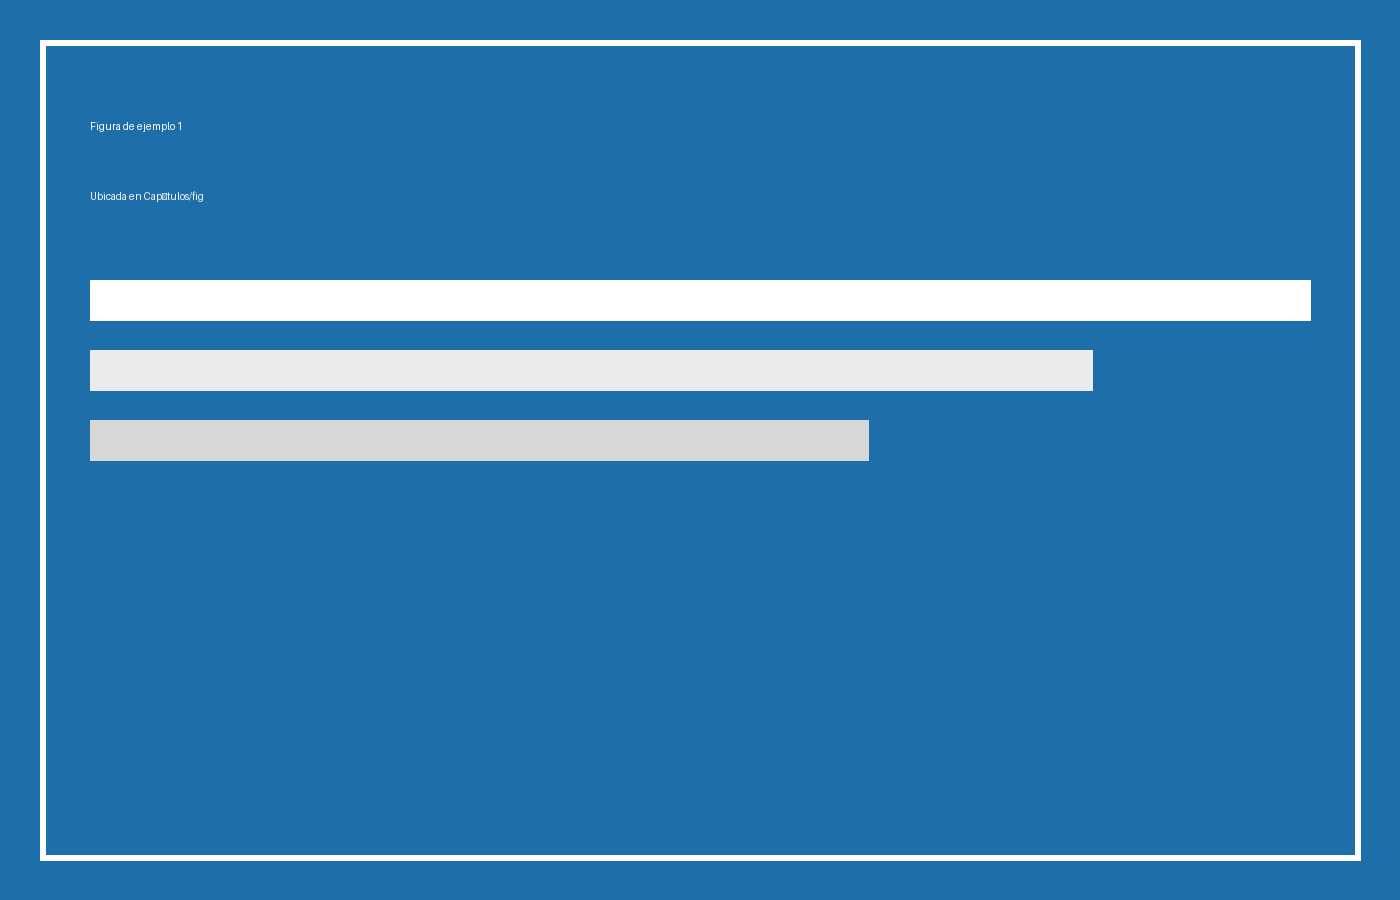
\includegraphics[width=0.80\textwidth]{Capítulos/fig/fig_ejemplo_1.png}
  \caption{Ejemplo de figura para guiar el formato de gráficos en el documento.}
  \label{fig:ejemplo_1}
\end{figure}
\elaboradopor{Estudiante}
\fuente{Elaboración propia}

\subsection{Ejemplo de Tabla 1}
Como ejemplo de referencia cruzada en párrafo: la Tabla~\ref{tab:ejemplo_1} resume indicadores base que luego pueden compararse con los resultados de implementación.

\begin{table}[htbp]
  \centering
  \caption{Ejemplo de tabla para registrar métricas iniciales del diagnóstico.}
  \label{tab:ejemplo_1}
  \begin{tabular}{|l|c|c|}
    \hline
    Indicador & Valor actual & Meta \\
    \hline
    Tiempo de respuesta (ms) & 850 & 400 \\
    \hline
    Disponibilidad (\%) & 96.2 & 99.0 \\
    \hline
    Incidencias mensuales & 14 & 6 \\
    \hline
  \end{tabular}
\end{table}
\elaboradopor{Estudiante}
\fuente{Datos de levantamiento inicial}
